\section{Optimization Techniques}
\label{sec:optimization}
Optimization is, undoubtedly, a crucial matter in the field of Data Science and Machine Learning. This section explores various
techniques stemming from optimization theory, aiming to enhance the performance of machine learning algorithms through the effective
minimization of loss functions. Starting from the fundamental principles of Gradient Descent, and continuing by presenting the key
variations relevant to this research approach, this analysis clarifies the role of optimizers in contemporary neural networks.

%%%%%%%%%%%%%%%%%%%%%%%%%%%%%%%%%%%%%%%%%%%%%%%%%%%%%%%%%%%%%%%%%%%%%%%%%%%%%%%%%%%%%%%%%%%%%%%%%%%%%%%%%%%%%%%%%%%%%%%%%%%%%%%%%%%%%%%%%%%%%%%%%%%%%%%%%%%%%%
\subsection{Gradient Descent And Its Variants}
\subsubsection{Principle of Gradient Descent}
Gradient Descent and its Variants are classified as iterative optimization algorithms, based on the idea of iteratively adjusting
the parameters (coefficients) of a model in the direction of the steepest descent with respect to the machine learning algorithm’s
cost function\cite{ruderOverviewGradientDescent2017}. Essentially, the objective of the algorithm is to find the parameter values
that minimize the cost function of the neural network. For this to be achieved, the gradient of the loss function at the current
point is calculated, indicating how small changes in the weights affect its output. Thus, the parameters are iteratively adjusted
in the opposite direction of the gradient—towards the minima point of the cost curve (see \cref{fig:gradient_descent}).

\begin{figure}[!ht]
    \centering
    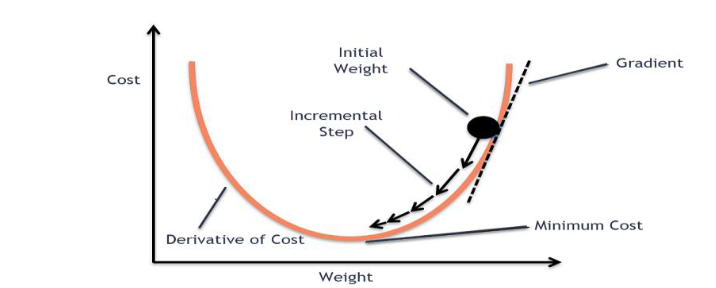
\includegraphics[width=.8\textwidth]{figures/opt/gradient_descent.png}
    \caption{Gradient Descent Algorithm\cite{hajiCOMPARISONOPTIMIZATIONTECHNIQUES2021}}
    \label{fig:gradient_descent}
\end{figure}

%%%%%%%%%%%%%%%%%%%%%%%%%%%%%%%%%%%%%%%%%%%%%%%%%%%%%%%%%%%%%%%%%%%%%%%%%%%%%%%
\subsubsection{Batch Gradient Descent}
Batch Gradient Descent (BGD), also referred to as Vanilla, computes the cost function with regard to the parameters $\theta$ for the
entire training dataset:
\begin{equation}
    \label{eq:bgd}
    \theta_{new} = \theta_{old} - \eta \cdot \nabla_{\theta} J(\theta)
\end{equation}

\noindent
Here, $\theta$ represents the parameters of the function to be minimized, $J(\theta)$ is the loss function, $\nabla_{\theta} J(\theta)$
denotes the gradient of the loss function with respect to $\theta$, and $\eta$ is the learning rate, which controls the size of the incremental
step taken towards the minimum.

Despite being easy to comprehend, BGD requires computing gradients for the entire dataset to update the model once, making it inefficient
for very large datasets or those exceeding memory capacity\cite{ruderOverviewGradientDescent2017}. Additionally, this method does not
support online updates with new data as it processes. Nonetheless, batch gradient descent is guaranteed to converge to the global minimum
for convex error surfaces and to a local minimum for non-convex surfaces.

%%%%%%%%%%%%%%%%%%%%%%%%%%%%%%%%%%%%%%%%%%%%%%%%%%%%%%%%%%%%%%%%%%%%%%%%%%%%%%%
\subsubsection{Stochastic Gradient Descent}
Proceeding with Stochastic Gradient Descent (SGD), this optimization method updates parameters incrementally for each training sample, $x^{(i)}$
and label $y^{(i)}$, unlike the previous discussion regarding BGD\@.

\begin{equation}
    \label{eq:sgd}
    \theta_{new} = \theta_{old} - \eta \cdot \nabla_{\theta} J(\theta; x^{(i)}; y^{(i)})
\end{equation}

The term stochastic in the name refers to the random selection of one sample for the gradient calculation instead of the entirety
of the dataset. This approach has been proven particularly beneficial for large-scale datasets and online learning algorithms as
it aids in reducing training time. Other commonly discussed properties of SGD include the ability to effectively escape local minima,
improved model generalizability to unseen data, and the detailed rate of improvement due to the frequency of updates. At the same time,
this per-sample frequency of parameter updates also leads to fluctuations in the error rate, instead of a steady and controlled decrease.

%%%%%%%%%%%%%%%%%%%%%%%%%%%%%%%%%%%%%%%%%%%%%%%%%%%%%%%%%%%%%%%%%%%%%%%%%%%%%%%
\subsubsection{Mini-Batch Gradient Descent}
This approach of optimization fills the middle space between BGD and SGD, as Mini-Batch Gradient Descent (MBGD) strikes a balance
between the computational efficiency of the former and the stability of the latter. Instead of updating parameters using all or
only one of the training examples, Mini-Batch Gradient Descent uses a subset of \emph{n} training data to perform each update:

\begin{equation}
    \label{eq:mbgd}
    \theta_{new} = \theta_{old} - \eta \cdot \nabla_{\theta} J(\theta; x^{(i:i+n)}; y^{(i:i+n)})
\end{equation}

This approach reduces the variance of the parameter updates, which can lead to more stable convergence than SGD while being
significantly faster than using the full dataset as in Batch Gradient Descent. This method is particularly effective for training
on large datasets making use of highly optimized matrix operations common to state-of-the-art deep learning libraries, resulting
in great efficiency while computing the gradients. All the above have contributed greatly to making MBGD the first choice of
optimization when training neural networks, while sometimes this is the case even when SGD is reported as the optimization algorithm
as the term SGD is used also when mini-batches are employed.

%%%%%%%%%%%%%%%%%%%%%%%%%%%%%%%%%%%%%%%%%%%%%%%%%%%%%%%%%%%%%%%%%%%%%%%%%%%%%%%
%%%%%%%%%%%%%%%%%%%%%%%%%%%%%%%%%%%%%%%%%%%%%%%%%%%%%%%%%%%%%%%%%%%%%%%%%%%%%%%%%%%%%%%%%%%%%%%%%%%%%%%%%%%%%%%%%%%%%%%%%%%%%%%%%%%%%%%%%%%%%%%%%%%%%%%%%%%%%%
\subsection{Towards ADAM Optimizer}

\subsubsection{Learning Rate Selection}
The learning rate hyperparameter, often denoted as $\eta$, is undoubtedly one of the most crucial factors contributing to the
convergence of gradient-based optimization algorithms\cite{ruderOverviewGradientDescent2017}. It determines the incremental step
size of the algorithm towards the minimum of the cost function, as observed in \cref{fig:gradient_descent}. The importance of
balancing the hyperparameter's value cannot be overstated; too high a learning rate can cause the algorithm to overshoot the minimum,
while too low a learning rate can result in excessively slow convergence or getting stuck in local minima (see \cref{fig:learning_rate}).
Therefore, achieving balance in this situation suggests swift convergence to the minimum.

\begin{figure}[!ht]
    \centering
    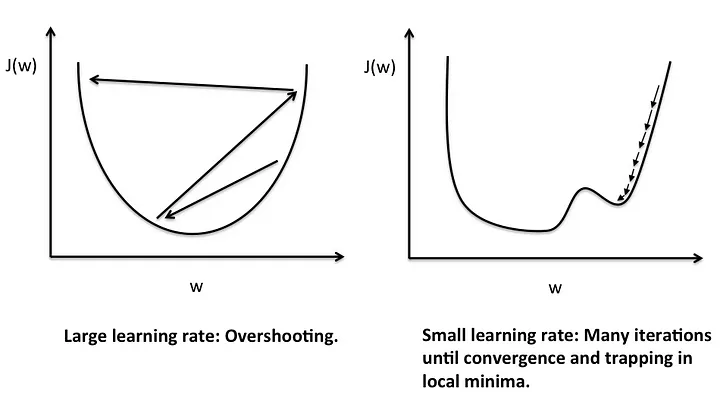
\includegraphics[width=.85\textwidth]{figures/opt/learning_rates_1.png}
    \caption{The effects of unsuccessful learning rate selection\cite{atulanandGRADIENTDESCENT2022}}
    \label{fig:learning_rate}
\end{figure}

%%%%%%%%%%%%%%%%%%%%%%%%%%%%%%%%%%%%%%%%%%%%%%%%%%%%%%%%%%%%%%%%%%%%%%%%%%%%%%%
\subsubsection{Momentum}
Momentum is an enhancement of Gradient Descent that accelerates convergence, particularly in the context of deep neural networks.
The term finds great applicability in situations where the network is not well-conditioned, leading to the composition of \emph{ravines}
—surfaces that curve more steeply in one direction than in another direction\cite{MomentumLearningRate,hajiCOMPARISONOPTIMIZATIONTECHNIQUES2021}.
Such surfaces negatively impact convergence, due to the simple fact that the gradient does not point towards the minimum, and successive
steps of gradient descent can oscillate from one side to the other, progressing, albeit very slowly, to the minimum. \Cref{fig:momentum}
illustrates how the addition of momentum aids in speeding up convergence to the minimum by damping these oscillations.

\begin{figure}[!ht]
    \centering
    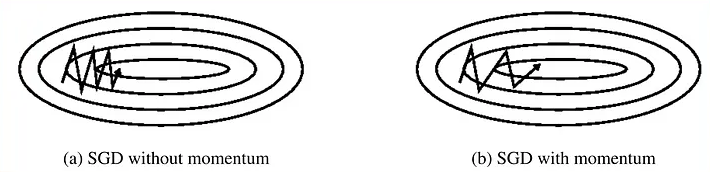
\includegraphics[width=.85\textwidth]{figures/opt/momentum.png}
    \caption{Trajectories in ravine surfaces, with and without momentum\cite{lecunEfficientBackProp1998}.}
    \label{fig:momentum}
\end{figure}

In the formal mathematical representation of SGD Momentum in \cref{eq:momentum}, $v_{t}$ represents the velocity, $\beta$ is the momentum
coefficient (typically set between 0.9 and 0.99), and $\nabla_{\theta} J(\theta; x^{(i)}; y^{(i)})$ is the gradient of the loss function.
In other words, the velocity that is calculated for a given moment $t$ complements the gradient descent calculation by taking into account
the momentum $\beta v_{t-1}$. This way, the update on the network's parameters is computed utilizing the velocity term that includes both
gradient and momentum.
\begin{equation}
    \begin{cases}
        v_{t} = \underbrace{\beta v_{t-1}}_{\text{momentum}} - \underbrace{\eta \cdot \nabla_{\theta} J(\theta; x^{(i)}; y^{(i)})}_{\text{gradient descent}} & \triangleright\text{ Velocity computation} \\
        \theta_{t} = \theta_{t-1} + v_{t}                                                                                                                    & \triangleright\text{ Parameters' update}
    \end{cases}
    \label{eq:momentum}
\end{equation}

%%%%%%%%%%%%%%%%%%%%%%%%%%%%%%%%%%%%%%%%%%%%%%%%%%%%%%%%%%%%%%%%%%%%%%%%%%%%%%%
\subsubsection{ADAM Optimizer}\label{sec:adam}
THe ADAM (Adaptive Moment Estimation) optimizer, proposed by Kingma and Ba (2017)\cite{kingmaAdamMethodStochastic2017}, is a widely utilized algorithm that combines
the benefits of both momentum and
adaptive learning rates, classifying it as an adaptive learning algorithm. This approach leverages concepts from Adagrad\cite{duchiAdaptiveSubgradientMethods}
and RMSprop\cite{LectureRmspropDivide}, making it particularly effective for deep neural network (DNN) training by managing
sparse gradients and non-stationary objectives.

By maintaining exponentially decaying averages, ADAM calculates adaptive learning rates of past gradients and squared gradients.
These moving averages smooth out noise in the gradient updates, providing a stable convergence path.
The momentum aspect, derived from the average of past gradients, helps accelerate convergence by maintaining
consistent update directions, thus reducing oscillations. Its implementation is summarized by \cref{alg:adam}:

In the following steps, $m_t$ and $v_t$ represent the first moment (mean) and second moment (uncentered variance) of the gradients,
respectively. The corrected estimates, $\hat{m}_t$ and $\hat{v}_t$, are used to compute the parameter updates. The decay rates $\beta_1$
and $\beta_2$ are typically set to 0.9 and 0.999, respectively, with $\epsilon$ preventing division by zero.

ADAM's ability to adaptively adjust learning rates for each parameter, based on the mean and variance of gradients, ensures robust performance
across various machine learning applications. This is especially beneficial for hyperparameter tuning and managing high-dimensional loss landscapes.

\begin{algorithm}[H]
    \caption{ADAM optimizer algorithm}
    \label{alg:adam}
    \begin{algorithmic}
        \Require $\alpha$: Stepsize
        \Require $\beta_1, \beta_2 \in [0, 1)$: Exponential decay rates for the moment estimates
        \Require $f(\theta)$: Stochastic objective function with parameters $\theta$
        \Require $\theta_0$: Initial parameter vector
        \Statex
        \Statex \textbf{Initialize:}
        \Statex $m_0 \leftarrow 0$ \Comment{Initialize 1\textsuperscript{st} moment vector}
        \Statex $v_0 \leftarrow 0$ \Comment{Initialize 2\textsuperscript{nd} moment vector}
        \Statex $t \leftarrow 0$ \Comment{Initialize timestep}
        \Statex
        \While{$\theta_t$ not converged}
        \Statex $t \leftarrow t + 1$
        \Statex $g_t \leftarrow \nabla_{\theta} f_t(\theta_{t-1})$ \Comment{Get gradients w.r.t.\ stochastic objective at timestep $t$}
        \Statex $m_t \leftarrow \beta_1 \cdot m_{t-1} + (1 - \beta_1) \cdot g_t$ \Comment{Update biased first moment estimate}
        \Statex $v_t \leftarrow \beta_2 \cdot v_{t-1} + (1 - \beta_2) \cdot g_t^2$ \Comment{Update biased second raw moment estimate}
        \Statex $\hat{m}_t \leftarrow m_t / (1 - \beta_1^t)$ \Comment{Compute bias-corrected first moment estimate}
        \Statex $\hat{v}t \leftarrow v_t / (1 - \beta_2^t)$ \Comment{Compute bias-corrected second raw moment estimate}
        \Statex $\theta_t \leftarrow \theta{t-1} - \alpha \cdot \hat{m}_t / (\sqrt{\hat{v}_t} + \epsilon)$ \Comment{Update parameters}
        \EndWhile
        \Statex \textbf{return} $\theta_t$ \Comment{Resulting parameters}
    \end{algorithmic}
\end{algorithm}

In the Federated Learning realm that is studied, ADAM's optimization techniques are crucial for enhancing convergence rates and model performance.
The decentralized nature of Federated Learning introduces challenges such as heterogeneous data distributions and communication constraints, as will be
discussed in subsequent sections.
ADAM's adaptive learning rate mechanism facilitates effective training across distributed nodes, overcoming data variability and ensuring
efficient global model convergence.
%%%%%%%%%%%%%%%%%%%%%%%%%%%%%%%%%%%%%%%%%%%%%%%%%%%%%%%%%%%%%%%%%%%%%%%%%%%%%%%
%%%%%%%%%%%%%%%%%%%%%%%%%%%%%%%%%%%%%%%%%%%%%%%%%%%%%%%%%%%%%%%%%%%%%%%%%%%%%%%%%%%%%%%%%%%%%%%%%%%%%%%%%%%%%%%%%%%%%%%%%%%%%%%%%%%%%%%%%%%%%%%%%%%%%%%%%%%%%%